\documentclass[aspectratio=169,10pt]{beamer}

% ---------------------------------------------------------------------------
% Quantathon CR 2026 -- Challenge 3
% Presentacion: Planteamiento y propuesta de solucion para el modelo de
% Fermi-Hubbard 2D (ladder 4x2)
% ---------------------------------------------------------------------------

\usetheme{Madrid}
\usecolortheme{default}
\setbeamertemplate{navigation symbols}{}
\setbeamertemplate{footline}[frame number]

\usepackage[utf8]{inputenc}
\usepackage[T1]{fontenc}
\usepackage{amsmath,amssymb}
\usepackage{braket}
\usepackage{booktabs}
\usepackage{tikz}
\usetikzlibrary{arrows.meta,positioning,decorations.pathreplacing,calc}

% ---- Paleta "cuantica" -------------------------------------------------
\definecolor{qDeep}{RGB}{35,32,90}
\definecolor{qMid}{RGB}{75,55,160}
\definecolor{qAccent}{RGB}{0,150,170}
\definecolor{qWarn}{RGB}{190,60,50}
\definecolor{qGray}{RGB}{90,90,95}

\setbeamercolor{structure}{fg=qMid}
\setbeamercolor{title}{fg=white,bg=qDeep}
\setbeamercolor{frametitle}{fg=white,bg=qDeep}
\setbeamercolor{palette primary}{fg=white,bg=qDeep}
\setbeamercolor{palette secondary}{fg=white,bg=qMid}
\setbeamercolor{palette tertiary}{fg=white,bg=qDeep}
\setbeamercolor{block title}{fg=white,bg=qMid}
\setbeamercolor{block body}{bg=qMid!8}
\setbeamercolor{block title alerted}{fg=white,bg=qWarn}
\setbeamercolor{block body alerted}{bg=qWarn!8}
\setbeamercolor{item}{fg=qAccent}
\setbeamerfont{frametitle}{series=\bfseries}

\newcommand{\good}[1]{\textcolor{qAccent}{\textbf{#1}}}
\newcommand{\warn}[1]{\textcolor{qWarn}{\textbf{#1}}}

\title[Fermi-Hubbard 2D: planteamiento y propuesta]{Modelo de Fermi-Hubbard 2D en una escalera $4\times2$}
\subtitle{Planteamiento del problema y propuesta de solucion}
\author{Quantathon CR 2026 -- QWorld Hackathon, Challenge 3}
\date{}

\begin{document}

% =============================================================
\begin{frame}
  \titlepage
\end{frame}

% =============================================================
\begin{frame}{Agenda}
  \tableofcontents
\end{frame}

\section{Contexto}

% =============================================================
\begin{frame}{Contexto: continuacion del Challenge 3}
  \begin{itemize}
    \item El Challenge 3 ya cuenta con un entregable \good{completo y reproducible}: el
      \textbf{Modelo de Ising con Campo Transverso (TFIM)}, comparando ED, Trotter
      (\texttt{guppylang} + Selene) y VQE (HEA) en \texttt{N=6} sitios.
    \item Este trabajo propone una \textbf{segunda instancia del mismo problema}, con un
      sistema fisicamente mas rico: el \textbf{modelo de Fermi-Hubbard en 2D}.
    \item Objetivo: mostrar que el enfoque \emph{ED vs.\ Trotter vs.\ VQE} generaliza a un
      Hamiltoniano fermionico, con un toolchain distinto (\textbf{Qiskit} en vez de
      guppylang/Selene) y honestidad sobre las dificultades nuevas que aparecen.
  \end{itemize}
  \vspace{1em}
  \begin{block}{Por que importa}
    Hubbard es el modelo de referencia para \textbf{correlaciones electronicas fuertes}
    (magnetismo, aislantes de Mott, superconductividad de alta $T_c$) -- un paso natural
    despues de un modelo de espines puro como TFIM.
  \end{block}
\end{frame}

\section{El modelo}

% =============================================================
\begin{frame}{Planteamiento: el Hamiltoniano de Hubbard}
  Para fermiones de espin $\sigma\in\{\uparrow,\downarrow\}$ sobre una red con enlaces
  $\langle i,j\rangle$:
  \[
    H = -t \sum_{\langle i,j\rangle,\sigma}\left(c^\dagger_{i,\sigma} c_{j,\sigma} + \text{h.c.}\right)
        \;+\; U \sum_i n_{i,\uparrow} n_{i,\downarrow}
        \;-\; \mu \sum_{i,\sigma} n_{i,\sigma}
  \]
  \begin{itemize}
    \item $t$: amplitud de \emph{hopping} (energia cinetica) $\leftrightarrow$ analogo de $J$ en TFIM.
    \item $U$: repulsion coulombiana en el mismo sitio $\leftrightarrow$ analogo de $h$ en TFIM.
    \item $\mu$: potencial quimico; $\mu = U/2$ fija \textbf{llenado medio} ($1$ fermion/sitio en promedio).
    \item Parametro barrido: $U/t$, con $t=1.0$ fijo -- mismo espiritu que el barrido de $h/J$ en TFIM.
  \end{itemize}
\end{frame}

% =============================================================
\begin{frame}{Nuestra red: escalera de Hubbard $4\times2$}
  \begin{columns}[T]
    \begin{column}{0.55\textwidth}
      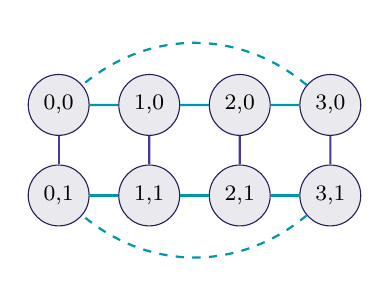
\begin{tikzpicture}[scale=1.15, every node/.style={circle,draw=qDeep,fill=qDeep!10,minimum size=7mm,font=\footnotesize}]
        \foreach \x in {0,1,2,3}{
          \node (t\x) at (\x,1) {\x,0};
          \node (b\x) at (\x,0) {\x,1};
        }
        % leg bonds (rows), interior
        \foreach \x/\y in {0/1,1/2,2/3}{
          \draw[qAccent,thick] (t\x) -- (t\y);
          \draw[qAccent,thick] (b\x) -- (b\y);
        }
        % wraparound leg bonds (arc outward, away from the ladder)
        \draw[qAccent,thick,dashed] (t3) to[bend right=40] (t0);
        \draw[qAccent,thick,dashed] (b3) to[bend left=40] (b0);
        % rung bonds
        \foreach \x in {0,1,2,3}{
          \draw[qMid,thick] (t\x) -- (b\x);
        }
      \end{tikzpicture}
      \vspace{0.3em}
      \small \textcolor{qAccent}{---} enlaces de pierna (\emph{leg}, periodico) \quad
      \textcolor{qMid}{---} enlaces de peldano (\emph{rung}, abierto)
    \end{column}
    \begin{column}{0.45\textwidth}
      \begin{itemize}
        \item $8$ sitios: $x=0..3$ (\textbf{periodico}), $y=0,1$ (\textbf{abierto}).
        \item $12$ enlaces vecino-cercano: $8$ de pierna $+$ $4$ de peldano.
        \item $2$ especies de espin $\Rightarrow$ $24$ terminos de hopping $+$ $8$ de interaccion.
        \item Llenado medio: $N_\uparrow=N_\downarrow=4$, $N=8$.
      \end{itemize}
    \end{column}
  \end{columns}
\end{frame}

% =============================================================
\begin{frame}{Honestidad fisica: \emph{crossover}, no transicion de fase}
  \begin{alertblock}{Lo que NO vamos a encontrar}
    Una escalera de 2 piernas es \warn{gapeada para todo $U>0$}: a $U/t$ grande el modelo
    efectivo es una escalera de Heisenberg cuyo estado base es un \textbf{singlete de peldano}
    con brecha de espin finita, conectado adiabaticamente hasta $U\to0^+$.
    \textbf{No existe un $U_c$ finito con transicion de fase} a llenado medio.
  \end{alertblock}
  \begin{block}{Lo que si vamos a caracterizar: un \emph{crossover} diagnosticado por}
    \begin{itemize}
      \item Doble ocupacion $\langle n_\uparrow n_\downarrow\rangle$: decrece de $1/4$ a $0$.
      \item Brecha de carga $\Delta_c(L) = E_0(N{+}1)+E_0(N{-}1)-2E_0(N)$: positiva para $U>0$.
      \item \textbf{Brecha de espin} $\Delta_s = E_0(S_{\text{tot}}{=}1) - E_0(S_{\text{tot}}{=}0)$:
        diagnostico propio de la escalera, crece con $U/t$.
      \item Correlacion de peldano $\langle \vec S_{(x,0)}\cdot\vec S_{(x,1)}\rangle$: se
        vuelve mas negativa al formarse los singletes.
    \end{itemize}
  \end{block}
\end{frame}

\section{De fermiones a qubits}

% =============================================================
\begin{frame}{Mapeo Jordan-Wigner: formulas base}
  Fijamos un orden lineal $1,\dots,M$ de los $M = 2\times8 = 16$ modos fermionicos
  (sitio $\times$ espin). Para el modo $j$:
  \[
    c_j = \Big(\prod_{k<j} Z_k\Big)\frac{X_j+iY_j}{2}, \qquad
    n_j = c_j^\dagger c_j = \frac{I-Z_j}{2} \quad \text{(siempre local)}
  \]
  Para dos modos $i<j$ (el termino de hopping):
  \[
    c^\dagger_i c_j + c^\dagger_j c_i = \frac{1}{2}\Big[X_i\big(Z_{i+1}\cdots Z_{j-1}\big)X_j
      + Y_i\big(Z_{i+1}\cdots Z_{j-1}\big)Y_j\Big]
  \]
  \begin{itemize}
    \item Es una compuerta ``$XX+YY$'' vestida con una \textbf{cadena de $Z$} sobre todo modo
      \emph{entre} $i$ y $j$ en el orden elegido.
    \item En 1D el orden fisico de la cadena ya es un orden JW valido $\Rightarrow$ vecinos
      cercanos = vecinos en el registro = \textbf{sin cadenas}. En 2D \warn{eso ya no es cierto}.
  \end{itemize}
\end{frame}

% =============================================================
\begin{frame}{El obstaculo central en 2D}
  \begin{block}{Ningun orden lineal deja todos los enlaces locales}
    Cualquier forma de aplanar una red 2D en una linea deja algunos pares fisicamente
    vecinos \textbf{lejos} en el registro $\Rightarrow$ esos hopping adquieren cadenas de $Z$
    no triviales. Es un costo \emph{inherente a la dimension}, que TFIM (1D) no tenia.
  \end{block}
  \textbf{Orden elegido:} por bloque de espin, y dentro de cada bloque \emph{row-major}:
  \[
    \underbrace{(0,0)_\uparrow \cdots (3,1)_\uparrow}_{\text{posiciones }0\text{--}7}
    \quad\Big|\quad
    \underbrace{(0,0)_\downarrow \cdots (3,1)_\downarrow}_{\text{posiciones }8\text{--}15}
  \]
  \centering
  \begin{tabular}{lccc}
    \toprule
    Tipo de enlace & Ejemplo & Distancia en registro & \textbf{Longitud de cadena} \\
    \midrule
    Pierna, interior & $(0,y)$--$(1,y)$ & adyacente & \good{0} \\
    Pierna, periodico & $(3,y)$--$(0,y)$ & 3 & \good{2} \\
    Peldano & $(x,0)$--$(x,1)$ & 4 & \warn{3} \\
    \bottomrule
  \end{tabular}
  \vspace{0.4em}
  \small Bloqueo por espin mantiene la interaccion $n_\uparrow n_\downarrow$ \good{siempre local}
  (producto de dos operadores de numero), aunque los dos qubits esten 8 posiciones aparte.
\end{frame}

\section{Circuito: Trotter}

% =============================================================
\begin{frame}{Capas de Trotter que conmutan}
  Agrupamos terminos en capas \textbf{mutuamente conmutantes} (enlaces que comparten qubit no
  conmutan entre si):
  \begin{columns}[T]
    \begin{column}{0.55\textwidth}
      \begin{itemize}
        \item \textbf{Pierna-par} (por espin): $\{(0,1),(2,3)\}$ en ambas filas -- 1 capa.
        \item \textbf{Pierna-impar} (por espin): $\{(1,2),(3,0)\}$ en ambas filas -- 1 capa.
        \item \textbf{Peldano} (por espin): los 4 enlaces son disjuntos -- 1 capa.
        \item \textbf{Interaccion}: los 8 terminos $n_\uparrow n_\downarrow$ son diagonales -- 1 capa.
      \end{itemize}
      \[
        \underbrace{3\times2}_{\text{hopping, 2 espines}} + \underbrace{1}_{\text{interaccion}}
        = \good{7 \text{ capas de Trotter}}
      \]
    \end{column}
    \begin{column}{0.45\textwidth}
      \small
      \begin{block}{Comparacion con TFIM}
        TFIM: 2 capas (ZZ par/impar $+$ X). \\
        Fermi-Hubbard: \warn{7 capas}, y las de peldano cargan cadenas de longitud 3 --
        mas CNOTs por paso que cualquier enlace de TFIM.
      \end{block}
    \end{column}
  \end{columns}
\end{frame}

% =============================================================
\begin{frame}{Costo y escala del problema}
  \centering
  \renewcommand{\arraystretch}{1.3}
  \begin{tabular}{lcc}
    \toprule
     & \textbf{TFIM} (resuelto) & \textbf{Fermi-Hubbard 2D} (propuesto) \\
    \midrule
    Sitios / qubits & 6 / 6 & 8 / \good{16} \\
    Dim. Hilbert & $2^6=64$ & $2^{16}=\good{65536}$ \\
    Capas de Trotter & 2 & \warn{7} \\
    Cadenas $Z$ & ninguna & 0, 2 o 3 qubits \\
    Ansatz VQE & HEA generico & \good{conserva $N$, $S_{\text{tot}}$} \\
    Toolchain & guppylang + Selene & \good{Qiskit} \\
    \bottomrule
  \end{tabular}
  \vspace{0.7em}
  \begin{alertblock}{Consecuencia practica}
    ED sigue siendo rutinaria, pero cada evaluacion de circuito (Trotter y, sobre todo, cada
    paso de VQE) es mas cara -- hay que presupuestar shots y \texttt{maxiter} con mas cuidado
    que en TFIM.
  \end{alertblock}
\end{frame}

\section{Propuesta de implementacion}

% =============================================================
\begin{frame}{Logica de implementacion: que se deriva a mano vs. que hace Qiskit}
  \begin{block}{Se deriva a mano (igual que en TFIM)}
    Hamiltoniano de red, mapeo Jordan-Wigner (\S2), agrupamiento en capas de Trotter (\S2.4) --
    \textbf{no} se usan los mappers automaticos de \texttt{qiskit-nature}.
  \end{block}
  \begin{block}{Qiskit aporta}
    Primitivas de circuito (\texttt{QuantumCircuit}, \texttt{PauliEvolutionGate} como bloque
    para un termino de Pauli ya especificado a mano), ejecucion (Aer), estimacion de valores
    esperados (\texttt{Estimator}) y el bucle de optimizacion clasica de VQE.
  \end{block}
  \small Mismo principio que en el notebook de TFIM: la fisica y la construccion del circuito
  son nuestras; el simulador/backend es prestado.
\end{frame}

% =============================================================
\begin{frame}{Plan por secciones (espejo de la estructura de TFIM)}
  \begin{enumerate}
    \item[\good{A}] \textbf{ED (linea base clasica)} -- Hamiltoniano en sector fijo
      $(N_\uparrow,N_\downarrow)$, \texttt{eigsh} disperso $\Rightarrow$ $E_0$, doble ocupacion,
      correlaciones de espin, y las brechas $\Delta_c,\Delta_s$ via sectores adyacentes.
    \item[B] \textbf{Trotter (Qiskit)} -- las 7 capas de \S2.4 como rotaciones
      $XX{+}YY$/$ZZ$ vestidas con las cadenas de \S2.3; dinamica de quench vs.\ referencia ED.
    \item[C] \textbf{Error de Trotter} -- convergencia del error en funcion de $\Delta t$,
      misma estructura que la Seccion C de TFIM.
    \item[D] \textbf{VQE} -- ansatz de compuertas de hopping / rotaciones de Givens que
      \textbf{conserva} $N$ y (idealmente) $S_{\text{tot}}$ -- un HEA generico exploraria
      sectores no fisicos.
    \item[] \textbf{Limitaciones} -- crossover vs.\ transicion, costo de cadenas $Z$ en 2D,
      ruido de shots, no-convergencia de VQE (igual honestidad que en TFIM).
  \end{enumerate}
\end{frame}

% =============================================================
\begin{frame}{Estado actual del proyecto}
  \begin{columns}[T]
    \begin{column}{0.5\textwidth}
      \textbf{\good{Hecho}}
      \begin{itemize}
        \item \texttt{fermi\_hubbard\_theory.md}: derivacion completa (Hamiltoniano, JW,
          capas de Trotter, plan por seccion).
        \item Seccion A implementada en
          \texttt{FermiHubbard2D\_ED\_Trotter\_VQE.ipynb}:
          \texttt{basis\_states}, \texttt{build\_fermi\_hubbard\_operators}, estado base y
          observables a llenado medio, barrido de crossover en $U/t$.
        \item Figura generada: \texttt{fermi\_hubbard\_2d\_phase\_diagram.png}.
      \end{itemize}
    \end{column}
    \begin{column}{0.5\textwidth}
      \textbf{\warn{Pendiente}}
      \begin{itemize}
        \item Agregar \texttt{qiskit} (+ \texttt{qiskit-aer}) a \texttt{requirements.txt} --
          hoy solo esta el stack de guppylang/Selene (para TFIM).
        \item Seccion B: circuito de Trotter (7 capas).
        \item Seccion C: barrido de convergencia de $\Delta t$.
        \item Seccion D: ansatz VQE que conserva numero de particulas.
        \item Seccion de limitaciones para el nuevo notebook.
      \end{itemize}
    \end{column}
  \end{columns}
\end{frame}

% =============================================================
\begin{frame}{Riesgos y mitigaciones}
  \centering
  \renewcommand{\arraystretch}{1.25}
  \begin{tabular}{p{0.42\textwidth}p{0.5\textwidth}}
    \toprule
    \textbf{Riesgo} & \textbf{Mitigacion} \\
    \midrule
    Costo de simulacion ($2^{16}$, 7 capas, VQE) & Reducir shots/\texttt{maxiter} para pruebas
      rapidas, igual que se hizo en TFIM \\
    Ansatz HEA generico rompe conservacion de $N$ & Usar ansatz de hopping/Givens
      restringido al sector fisico \\
    Interpretar mal un crossover como transicion & Reportar $\Delta_s$, $\Delta_c$ y
      correlaciones explicitamente, con el caveat del \S1.3 en el notebook \\
    Cadenas $Z$ largas $\Rightarrow$ mas ruido/CNOTs & Documentar el costo (tabla \S2.3) y
      citar SWAP networks como camino de escalamiento futuro \\
    \bottomrule
  \end{tabular}
\end{frame}

\section{Cierre}

% =============================================================
\begin{frame}{Resumen}
  \begin{itemize}
    \item El problema esta \good{completamente planteado}: Hamiltoniano, mapeo JW, costo de
      cadenas por enlace, capas de Trotter, y observables de crossover -- todo derivado a mano
      en \texttt{fermi\_hubbard\_theory.md}.
    \item La \good{linea base clasica (ED)} ya esta implementada y reproducible.
    \item Existe un \good{plan concreto y acotado} para las secciones B, C y D, siguiendo la
      misma estructura ya validada con TFIM pero con un toolchain (Qiskit) y un ansatz
      adaptados a la fisica fermionica.
    \item El trabajo es \good{honesto sobre sus limites}: crossover (no transicion), costo
      2D de Jordan-Wigner, y el tamano de sistema que efectivamente se puede simular.
  \end{itemize}
  \vfill
  \centering \large \textcolor{qDeep}{\textbf{Gracias -- preguntas}}
\end{frame}

\end{document}
